\documentclass[11pt]{article}
%Gummi|065|=)
\title{\textbf{Pathfinding su giochi grid-based}}
\author{Lentisco Francesco\\
N86001092}
\date{}
\usepackage{graphicx}
\usepackage[linesnumbered,algoruled,boxed,lined]{algorithm2e}
\usepackage{float}
\usepackage{fancyvrb}
\usepackage{cprotect}
\usepackage{listings}
\usepackage{color}
\begin{document}

\maketitle

\section{Le Mappe}

Un gioco grid-based (o tile-based) \`e un tipo di videogioco dove l'area di gioco consiste in piccole immagini grafiche rettangolari, quadrate o esagonali, note come \emph{tiles}. L'insieme completo dei \emph{tile} disponibili per l'area di gioco \`e chiamato \emph{tileset}. I \emph{tile} sono disposti in maniera adiacente l'uno dall'altro nella griglia. I giochi \emph{tile-based} di solito simulano una veduta dall'alto (\emph{top-down}) dell'area di gioco e sono generalmente bidimensionali. \par Nel progetto proposto ci si \`e serviti di mappe \emph{grid-based} generate in modo randomico a seconda del \emph{pattern} desiderato. La mappa consiste in una griglia con larghezza e altezza fissate ed ogni cella (\emph{tile}) puo' essere bloccata o traversabile. L'implementazione dei grafi usati per costruire il sistema di navigazione di ogni mappa \`e fornita dalla libreria \emph{JGrapht}\footnote{http://jgrapht.org/}. \par Ogni \emph{tile} della mappa corrisponde ad un nodo nel grafo corrispondente. Ogni nodo \`e connesso con tutti i nodi associati ai \emph{tile} adiacenti e non bloccati (in 8 direzioni). I \emph{tile} non attraversabili sono associati a un nodo con zero archi entranti. I pesi degli archi ortogonali hanno un costo unitario, pertanto gli archi tra due nodi collegati diagonalmente hanno un costo di $\sqrt{2}$. \par Per riferirsi a un nodo del grafo partendo dalle sue coordinate sulla grigla e viceversa si usano delle semplici formule di conversioni:
siano x e y le cordinate geometriche del nodo del grafo che si vuole referenziare\begin{equation} nodo = y*MAP\_WIDTH + x \end{equation} dove \emph{MAP\_WIDTH} si intende la larghezza della mappa. Per convertire invece un nodo del grafo nelle sue coordinate geometriche si utilizzano le seguenti: \begin{equation} x = nodo \% MAP\_WIDTH \end{equation} \begin{equation} y = nodo / MAP\_WIDTH \end{equation} \par Le mappe possono essere generate secondo 3 diversi \emph{pattern} di generazione al fine di rappresentare lo stile delle mappe tipiche dei retro game.

\subsection{Mappe \emph{Hallways}}
\begin{figure}[htp]
\centering
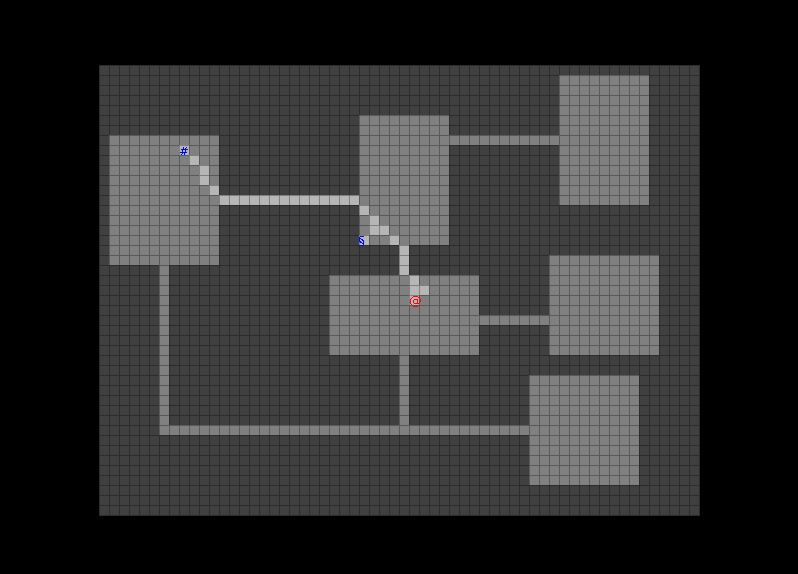
\includegraphics[scale=0.30]{/home/notsaved/Documenti/2dgrid-game/DijkstraDungeon.png}
\caption{mappa \emph{Hallways}}
\label{img1}
\end{figure}
%Support for two high-level {\LaTeX} building systems, \emph{rubber}\footnote{https://launchpad.net/rubber/} \& \emph{latexmk}\footnote{http://www.phys.psu.edu/{\textasciitilde}collins/software/latexmk-jcc/} has been added as well. Your preferred typesetter can be configured through the Compilation tab in the Preferences menu. Typesetters that are not installed on your system will not be selectable. 
Questo tipo di mappa si compone di grandi stanze collegate da lunghi corridoi. Una classe \emph{stanza} e' cosi' definita:

\lstdefinestyle{customjava}{
  belowcaptionskip=1\baselineskip,
  breaklines=true,
  frame=L,
  xleftmargin=\parindent,
  language=java,
  showstringspaces=false,
  basicstyle=\footnotesize\ttfamily,
  keywordstyle=\bfseries\color{black},
  commentstyle=\itshape\color{black},
  identifierstyle=\color{blue},
  stringstyle=\color{orange},
}
\lstset{style=customjava, caption=Classe java "\emph{Room}"}
\begin{lstlisting}
public class Room implements TileMapElement{
	private int x, y, width, height, area;

	public Room(int x,int y, int width, int height){
		this.x=x;
		this.y=y;
		this.width=width;
		this.height=height;
		this.area=width*height;
	}
}

\end{lstlisting}
Una stanza consiste in un rettangolo di \emph{Tile} traversabili. Gli attributi \emph{x} e \emph{y} sono le coordinate dell'angolo in basso a sinistra della stanza mentre \emph{width} e \emph{height} rispettivamente larghezza e altezza della stanza (espressi in numero di \emph{Tile}). Tale classe e' inoltre dotata di un metodo \emph{intersect()} cos\`i definito:

\lstdefinestyle{customjava}{
  belowcaptionskip=1\baselineskip,
  breaklines=true,
  frame=L,
  xleftmargin=\parindent,
  language=java,
  showstringspaces=false,
  basicstyle=\footnotesize\ttfamily,
  keywordstyle=\bfseries\color{black},
  commentstyle=\itshape\color{black},
  identifierstyle=\color{blue},
  stringstyle=\color{orange},
}
\lstset{style=customjava, caption=Funzione \emph{Intersect}}
\begin{lstlisting}
public boolean intersect(Object other){
    if(other.getClass()!=Room.class)
        return false;
    Room r = (Room) other;
    return !(this.x+ this.width < r.x 
        || r.x + r.width < this.x 
        || this.y+this.height < r.y 
        || r.y + r.height < this.y);
}

\end{lstlisting}

 L'algoritmo utilizzato per la generazione di questo tipo di mappa prende in ingresso una griglia di interi interamente riempita di 1, ossia totalmente riempita di \emph{Tile} non traversabili. In seguito sceglie in modo randomico (ma di un certo range prestabilito) la posizione e la grandezza delle stanze da posizionare nella mappa. Le stanze vengono scelte in modo da non sovrapporsi. Infine, dopo aver posizionato tutte le stanze, l'algoritmo provvedera' a connettere tutte le stanze creando dei tunnel ortogonali da una stanza a un'altra riempendo di zeri la griglia nelle coordinate dei punti che compongono il tunnel. L'algoritmo utilizzato e' il seguente:\par
\SetKwProg{Fn}{Function}{}{}
\begin{algorithm}[H]
\PrintSemicolon
\caption{Hallways map generator}
\KwData{MAX\_ROOM\_SIZE: integer, MIN\_ROOM\_SIZE: integer, MAX\_ROOMS: integer,  rooms: list of \emph{Room} object}
\KwIn{Array bidimensionale di interi con dimensioni \emph{WIDTH} x \emph{HEIGHT}}
\KwResult{L'array bidimensionale in ingresso viene elaborato in una mappa}
\newcommand{\forcond}{$i=0$ \KwTo $n$}

\Fn{main (map)}{


 \For{$i=0$ \KwTo $MAX\_ROOMS$}{
 \tcc{assegno le dimensioni della stanza e la sua posizione randomicamente}
  $w$ $\leftarrow$ \textbf{random}(((ROOM\_MAX\_SIZE - ROOM\_MIN\_SIZE) + 1) + ROOM\_MIN\_SIZE\;
  $h$ $\leftarrow$ \textbf{random}(((ROOM\_MAX\_SIZE - ROOM\_MIN\_SIZE) + 1) + ROOM\_MIN\_SIZE\;
  $x$ $\leftarrow$ \textbf{random}(WIDTH - W - 1) + 1\;
  $y$ $\leftarrow$ \textbf{random}(HEIGHT - H - 1) + 1\;
  $room$ $\leftarrow$ \textbf{new} Room(w,h,x,y)\;
  $noGood$ $\leftarrow$ false\;
  \For{$r\in rooms$ \tcc{controllo che non ci siano sovrapposizioni con le stanze gia' presenti}}{
  	\If{$room.\textbf{intersect}(r)$}{
  		$noGood$ $\leftarrow$ true\;
  		\textbf{break\;}}
  }
  \If{$!noGood$ \tcc{riempio di zeri la griglia nelle coordinate corrispondenti alla stanza}}{
  \For{$i = room.X$ \KwTo $(room.X + room.W)$ }{
  \For{$j = room.Y$ \KwTo $(room.Y + room.H)$ }{
  $map_{ij}$ $\leftarrow$ 0\;
  }}
  $rooms.\textbf{add}(room)$\;}

 }
  $\textbf{createTunnels}(map)$;\ \tcc{connetti le stanze create}

}
\end{algorithm}

\begin{algorithm}
  \LinesNumbered
\setcounter{AlgoLine}{26}
%This is to hide Begin keyword
\SetKwBlock{Begin}{}{end}
 \Fn{createTunnels(map)}{
 	$prev \longleftarrow \emptyset$\;
 	\For{$r\in rooms$ }{
 	\If{$r.\textbf{hasPrev}()$}{
 	$prev \longleftarrow r.prev$\;
 	\If{\textbf{random}(\textbf{range}(0,100)) $>$ 50 \tcc{decido casualmente se creare prima un tunnel orizzontale e poi verticale o viceversa}}{
 	$\textbf{createHorizontalTunnel}(\begin{tabular}{@{\hspace*{1.0em}}l@{}}
map, prev.\textbf{getCenterX}() \\
   	r.\textbf{getCenterX}(), prev.\textbf{getCenterY}()\end{tabular})$\;
 	$\textbf{createVerticalTunnel}(\begin{tabular}{@{\hspace*{1.0em}}l@{}}
map, prev.\textbf{getCenterY}() \\
   	r.\textbf{getCenterY}(), r.\textbf{getCenterX}()\end{tabular})$\;
 	}
 	\Else{
 	$\textbf{createVerticalTunnel}(\begin{tabular}{@{\hspace*{1.0em}}l@{}}
map, prev.\textbf{getCenterY}() \\
   	r.\textbf{getCenterY}(), prev.\textbf{getCenterX}()\end{tabular})$\;
 	$\textbf{createHorizontalTunnel}(\begin{tabular}{@{\hspace*{1.0em}}l@{}}
map, prev.\textbf{getCenterX}() \\
   	r.\textbf{getCenterX}(), r.\textbf{getCenterY}()\end{tabular})$\;
 	}
 	}
 	}

 }

 \Fn{createHorizontalTunnel(map, x1, x2, y)}{
 	\For{$i=\textbf{min}(x1,x2)$ \KwTo $\textbf{max}(x1,x2)$}{
 	 	$map_{i,y} \leftarrow 0$\;}
 }
  \Fn{createVerticalTunnel(map, y1, y2, x)}{
   	\For{$j=\textbf{min}(y1,y2)$ \KwTo $\textbf{max}(y1,y2)$}{
 	 	$map_{x,j} \leftarrow 0$\;}
 }
  
\end{algorithm}



\subsection{Mappe \emph{Outdoor}}
\begin{figure}[htp]
\centering
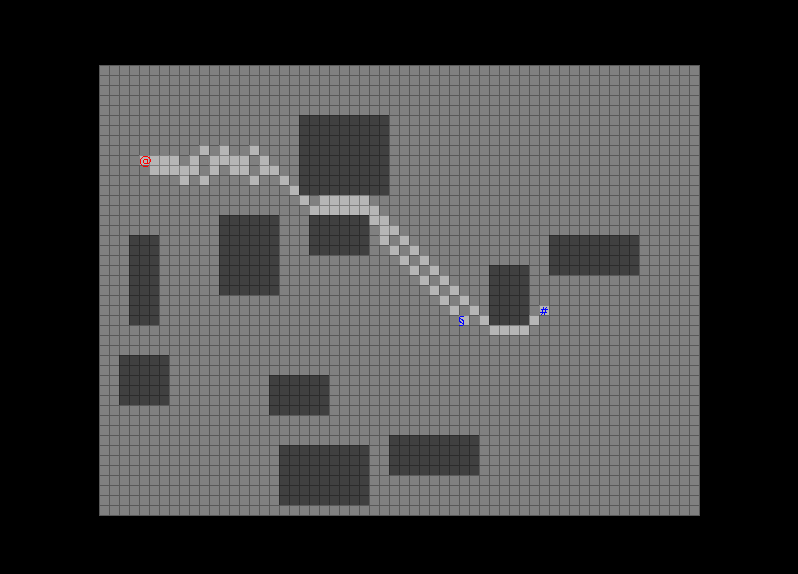
\includegraphics[scale=0.30]{/home/notsaved/Documenti/2dgrid-game/DijkstraOutdoor.png}
\caption{mappa \emph{Outdoor}}
\label{img2}
\end{figure}
Questo tipo di mappa, in maniera speculare al tipo di mappa della sezione precedente, si caratterizza da una griglia completamente riempita da \emph{Tile} traversabili dove vengono posizionati casualmente degli ostacoli rettangolari composti da \emph{Tile} non attraversabili di dimensioni a loro volta casuali.
Cos\`i come le stanze del tipo di mappa precedente, anche gli ostacoli di questo tipo di mappa non si sovrappongono. L'algoritmo utilizzato e' del tutto simile e speculare a quello di generazione delle mappe di tipo \emph{dungeon} eccetto per la creazione dei tunnel.
%Added for your viewing convenience is a continuous preview mode for the PDF. This mode is enabled by default, but can also be disabled through the \emph{(View $\rightarrow$ Page layout in preview)} menu. Complementary to this feature is SyncTeX integration, which allows you to synchronize the position in your editor with the PDF preview. 
\subsection{Mappe \emph{Indoor}}
\begin{figure}[H]
\centering
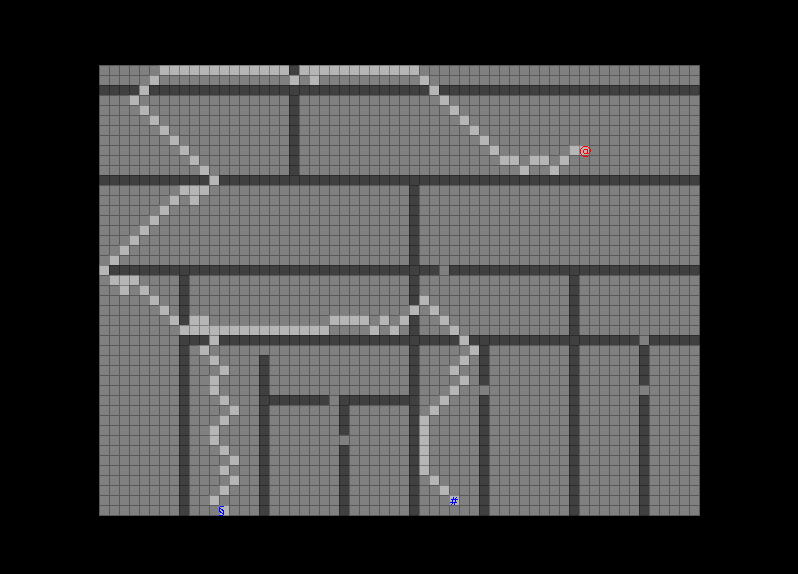
\includegraphics[scale=0.30]{Documenti/2dgrid-game/DijkstraIndoor.png}
\caption{mappa Indoor}
\label{img3}
\end{figure}

\par L'ultimo tipo di mappa realizzato consiste in uno spazio partizionato in diversi sottospazi (o stanze) servendosi di \emph{tile} non traversabili come \emph{muri} divisori. Le stanze sono raggiungibili da altre stanze mediante un \emph{tile} che viene lasciato attraversabile in ogni muro divisore. L'algoritmo utilizzato altro non \`e che una variante dell'algoritmo della divisione ricorsiva dello spazio. A seconda dell'orientamento, esso divide la griglia orizzontalmente o verticalmente disegnando un muro divisore e scegliendo un punto casuale su di esso dove posizionare il passaggio. In seguito divider\`a ricorsivamente i due sottospazi partizionati, finch\`e  non verra' raggiunto il caso base della ricorsione, ossia quando le stanze avranno dimensioni minori del minimo ammissibile.
\newcommand\And{\textbf{and}}
\begin{algorithm}[H]
\PrintSemicolon
\caption{indoor map generator}
\KwData{ROOM\_MIN\_SIZE: integer}
\KwIn{\;
Array bidimensionale di interi con dimensioni \emph{WIDTH} x \emph{HEIGHT} di soli zeri
\; offset di x e y
\; larghezza ed altezza della stanza
\; orientamento della divisione da effettuare}
\KwResult{L'array bidimensionale in ingresso viene elaborato in una mappa di tipo indoor}
\newcommand{\forcond}{$i=0$ \KwTo $n$}

\Fn{\textbf{divide} (map, x\_offset, y\_offset, width, height, orientation)}{

	\If{$(width < ROOM\_MIN\_WIDTH)$ \textbf{OR} $(heigth < ROOM\_MIN\_HEIGHT)$}{\Return\;}
\tcc{divido orizontalmente o verticalmente}
	$horizontal \leftarrow orientation == true$\;
\tcc{scelgo da dove comincera' il muro}

\If{$horizontal$}{
	$wx \leftarrow x\_offset$\;
	$wy \leftarrow y\_offset + random(height - 2)$\;
	}
\Else{
	$wx \leftarrow x\_offset + random(width - 2)$\;
	$wy \leftarrow y\_offset$\;
	}

\tcc{scelgo un punto lungo il muro da usare come passaggio}

\If{$horizontal$}{
	$px \leftarrow wx + random(width)$\;
	$py \leftarrow wy$\;
	}
\Else{
	$px \leftarrow wx$\;
	$py \leftarrow wy + random(height)$\;
	}
\tcc{scelgo la lunghezza del muro}
\If{$horizontal$}{
	$lenght \leftarrow width$\;
	}
\Else{
	$lenght \leftarrow height$\;
	}


}
\end{algorithm}


\begin{algorithm}
  \LinesNumbered
\setcounter{AlgoLine}{27}
%This is to hide Begin keyword
\SetKwBlock{Begin}{}{end}

\Begin{
\tcc{disegno il muro}
	\If{$horizontal$}{
		$dx \leftarrow 1$\;
		$dy \leftarrow 0$\;
		}
	\Else{
		$dx \leftarrow 0$\;
		$dy \leftarrow 1$\;
	}
	\For{$i=0$ \KwTo $lenght$}{
		\If{$wx \neq px$ \textbf{AND} $wy \neq py$}{
			$map_{wx,wy} \leftarrow 1$\;
		}
		$wx \leftarrow wx + dx$\;
		$wy \leftarrow wy + dy$\;
	}
	$nx \leftarrow x\_offset$\;
	$ny \leftarrow y\_offset$\;
	\tcc{se ho diviso orizzontalmente, dividi al di sopra del muro e poi al di sotto. Altrimenti prima a sinistra e poi a destra}
	
	\If{$horizontal$}{
		$new\_width \leftarrow width$\;
		$new\_height \leftarrow wy - y\_offset + 1$\;
		}
	\Else{
		$new\_width \leftarrow wx - x\_offset + 1$\;
		$new\_height \leftarrow height$\;
	}
	$\textbf{divide}(map, nx, ny, new\_width, new\_height, w < h)$\;
	\If{horizontal}{
	$nx \leftarrow x_offset$\;
	$ny \leftarrow wy +1$\;
	$new\_width \leftarrow width$\;
	$new\_height \leftarrow y\_offset + height - wy - 1$\;}
\Else{
	$nx \leftarrow wx + 1$\;
	$ny \leftarrow y\_offset$\;
	$new\_width \leftarrow x\_offset + width - wx - 1$\;
	$new\_height \leftarrow height$;}
$\textbf{divide}(map, nx, ny, new\_width, new\_height, w < h)$\;
}

  
\end{algorithm}







\section{Algoritmi di pathfinding}
\par{Il \emph{path-planning} \`e un componente fondamentale della maggior parte dei videogiochi.
Gli \emph{agent} spesso si muovono nell'area di gioco. A volte questo movimento \`e fissato dagli sviluppatori del gioco, come ad esempio il percorso di pattugliamento di un area che una guardia deve seguire. I percorsi fissi sono semplici da implementare, ma possono essere facilmente ingannati, ad esempio se un oggetto si frappone nel percorso. \emph{Agent} pi\`u complessi non sanno in anticipo dove dovranno muoversi. Una unit\`a in un gioco di strategia in tempo reale potrebbe ricevere l'ordine dal giocatore di muoversi in qualsiasi punto sulla mappa, oppure, in un gioco \emph{tile-based} pu\`o succedere che un agent debba inseguire il giocatore nell'area di gioco.
Per ognuna di queste situazioni, l'IA deve essere in grado di computare un percorso adeguato attraverso l'area di gioco per arrivare a destinazione, partendo dalla posizione attuale dell'agent. Inoltre vorremmo che il percorso trovato sia il pi\`u breve possibile.}
\par{La maggior parte dei giochi usa delle soluzioni di pathfinding basate sull'algoritmo chiamato A*. Nonostante sia molto semplice da implementare ed efficiente, A* non pu\`o lavorare direttamente sulla geometria del livello di gioco. Esso richiede che l'area di gioco sia rappresentata in una particolare struttura dati: un grafo diretto pesato e non-negativo.
In questo capitolo introdurremo la struttura dati grafo e in seguito verranno presentati tutti gli algoritmi implementati nel progetto, tra cui Dijkstra, A* e diverse sue varianti.}

\subsection{Dijkstra}
\par{
L'algoritmo di Dijkstra \`e un algoritmo utilizzato per cercare i cammini minimi (o Shortest Paths, SP) in un grafo con o senza ordinamento, ciclico e con pesi non negativi sugli archi.
Tale algoritmo non \`e stato progettato per il pathfinding nel senso inteso nei videogochi (\emph{point-to-point)}, ma piuttosto per risolvere il problema dei \emph{cammini minimi}.}

\par{Mentre nei videogiochi usualmente si computa il percorso minimo da un punto di partenza a un punto di arrivo, l'algoritmo di Dijkstra \`e realizzato in modo da trovare il percorso pi\`u breve da un punto di partenza verso tutti i restanti punti.
La soluzione includer\`a ovviamente anche l'eventuale punto di arrivo, ma ci\`o comporter\`a in ogni caso uno spreco di risorse computazionali se siamo interessati a un solo punto di arrivo.
Tuttavia pu\`o essere modificato in modo da generare solo il percorso nel quale siamo interessati, ma sar\`a ancora inefficiente come algoritmo di pathfinding.
}
\par{
Dijkstra \`e un algoritmo iterativo. Ad ogni iterazione, considera un nodo nel grafo ed esamina i suoi archi uscenti (nella prima iterazione considera il nodo di partenza). Ci riferiremo per semplicit\`a al nodo considerato in ogni iterazione come "nodo corrente".
Per ogni arco esamina il suo nodo terminale e memorizza il costo totale del cammino percorso fino ad arrivare ad esso (\emph{cost-so-far)} insieme all'arco dal quale si \`e arrivati in apposite strutture dati. Per quanto riguarda la prima iterazione, il nodo corrente \`e il nodo di partenza e il costo totale per ogni sua connessione \`e semplicemente il costo di quella connessione.
Dopo la prima iterazione, il costo totale del cammino per il nodo terminale di ogni connessione del nodo corrente, \`e uguale alla somma del costo totale del nodo corrente e del peso della connessione verso il nodo terminale.
}
\par{
L'algoritmo tiene traccia dei nodi da visitare in una coda di priorit\`a. La priorit\`a viene stabilita sulla base del costo totale del cammino associato a quel nodo. Nella prima iterazione la coda conterr\`a solo il nodo di partenza con costo totale uguale a 0. Nelle successive iterazioni l'algoritmo estrae dalla coda il nodo con il minor costo totale. Questo sar\`a processato come \emph{nodo corrente}.
}
\par{
Ogni volta che viene esaminato un nodo terminale, l'algoritmo confronter\`a il suo costo totale attuale (all'inizio tutti i nodi vengono inizializzati, assegnandoli un valore di costo di default pari a \emph{infinito}) con quello appena calcolato. Se il costo totale appena calcolato \`e minore di quello precedentemente assegnato a quel nodo terminale, tale valore viene aggiornato. Ovviamente oltre al valore di costo totale viene aggiornato anche il suo predecessore, che diventer\`a l'arco che connette il nodo corrente a quello terminale in esame. Quando si verifica questa condizione significa che l'algoritmo ha trovato un percorso migliore verso quel nodo terminale.
}
\par{
L'implementazione canonica di Dijkstra termina quando la coda \`e vuota, ossia, quando tutti i nodi appartenenti al grafo sono stati visitati e processati. Tuttavia per risolvere un problema di pathfinding, l'algoritmo pu\`o terminare prima che tutti i nodi vengano processati, ossia, quando il nodo di arrivo \`e il nodo con la priorit\`a pi\`u bassa nella in coda.
}
\par{
Una volta raggiunto il nodo di arrivo, viene estratto il cammino percorrendo a ritroso tutte le connessioni usate per arrivare a quel nodo fino a raggiungere il nodo di partenza.
}

\begin{algorithm}
\PrintSemicolon
\caption{Dijkstra Shortest Path}
  \LinesNumbered
%This is to hide Begin keyword
 \Fn{DijkstraShortestPath(Graph, source)}{
 	\tcc{array per tenere traccia del costo totale del percorso fino a quel nodo}
 	$dist[source] \longleftarrow 0 $\; 
 	\tcc{coda di priorit\`a}
 	 $Q \longleftarrow \emptyset$\;
 	\ForEach{$v \in Graph.\textbf{vertexSet}()$ }{
		\If{v $\neq$ source}{
		 	 $dist[v] \longleftarrow \infty$\;
		 	 $prev[v] \longleftarrow \emptyset$\;
		}
		$Q.\textbf{add}(v, dist[v])$\;
 	}
	\While{!Q.\textbf{isEmpty}()}{
		$u \longleftarrow Q.\textbf{extractMin}()$\;
		\ForEach{neighbor v of u}{
			$alt \longleftarrow dist[u] + \textbf{lenght}(u,v)$\;
			\If{alt \textless dist[v]}{
					 	 $dist[v] \longleftarrow alt$\;
					 	 $prev[v] \longleftarrow u$\;
					 	 $Q.\textbf{decreasePriority}(v,alt)$\;
			}
		}
	}
 } 
\end{algorithm}


\par{
Tenendo presente che la coda di priorit\`a \`e implementata come uno \emph{heap di Fibonacci} e che la complessit\`a delle operazioni di \textbf{extractMin}() e \textbf{decreasePriority}() sono rispettivamente $\mathcal{O}(log(n))$ e $\Theta(1)$, la complessit\`a dell'algoritmo nel caso peggiore \`e di $\mathcal{O}(|E| + |V| \log|V|)$.
}
\subsection{A*}
La maggior parte dei sistemi di \emph{pathfinding} odierni sono basati su questo algoritmo, data la sua efficienza, semplicit\`a di implementazione e ampi margini di ottimizzazione.
Diversamente dall'algoritmo di Dijkstra, A* \`e pensato per la ricerca del percorso minimo \emph{point-to-point}.
\par{
Il funzionamento dell'algoritmo \`e molto simile a quello di Dijkstra. A differenza di quest'ultimo, che sceglie sempre prima il nodo con il minor \emph{cost-so-far}, A* sceglier\`a il nodo candidato che \emph{pi\`u probabilmente} porter\`a al pi\`u breve percorso. Questa nozione di probabilit\`a \`e data da funzioni \emph{euristiche}. Pi\`u la funzione euristica utilizzata sar\`a accurata, pi\`u l'algoritmo sar\`a efficiente
}
\par{
A* funziona iterativamente: in ogni iterazione considera un nodo del grafo ed esamina le sui archi uscenti. Il nodo corrente viene scelto usando un criterio di selezione simile a quello di Dijkstra, ma con la significativa differenza dell'euristica.
}
\par{
Per ogni arco uscente dal nodo corrente, A* esamina il suo nodo terminale e memorizza il costo totale del cammino percorso fino ad arrivare ad esso (\emph{cost-so-far)} insieme all'arco dal quale si \`e arrivati in apposite strutture dati, esattamente come Dijkstra. Inoltre A* memorizza un valore in pi\`u: una stima euristica del costo totale del percorso(\emph{f(x)}), passando per quel nodo, dal nodo di partenza al nodo di arrivo. Questo costo totale stimato \`e la somma di due valori: il costo totale (\emph{cost-so-far}, da questo punto in poi ci riferiremo a questo valore come \emph{g(x)}) di quel nodo e la distanza (euristica) dal nodo in esame fino al nodo di arrivo. Questa stima \`e tipicamente generata da una funzione euristica che di solito non fa parte dell'algoritmo stesso.
}
\par{
Queste stime sono chiamate \emph{valori euristici} e ci riferiremo per semplicit\`a a essi come \emph{h(x)}. Pertanto \emph{f(x) = g(x) + h(x)}.
}
\par{
A* tiene traccia dei nodi visitati ma ancora da processare in una coda, a cui ci riferiremo come \emph{Open}, e dei nodi gi\`a processati in una lista \emph{Closed}. I nodi saranno inseriti nella coda \emph{Open} appena saranno scoperti lungo gli archi uscenti dal nodo corrente. Essi verranno successivamente trasferiti nella lista \emph{Closed} alla fine della loro stessa iterazione.
}
\par{Diversamente da Dijkstra, viene estratto dalla coda \emph{Open} il nodo con il minor valore \emph{f(x)}. Questa variazione permette di valutare per primi i nodi pi\`u promettenti. Se la stima \`e accurata allora i nodi che sono pi\`u vicini al nodo di arrivo vengono considerati per prima, restringendo il campo di ricerca nelle aree pi\`u proficue.}
\par{Potrebbe accadere che si arrivi ad esaminare un nodo appartenente alla coda \emph{Open} o alla lista \emph{Closed} e si debbano modificare i suoi valori di costo. In questo caso calcoleremo il valore \emph{g(x)} come al solito e se esso \`e minore di quello gi\`a memorizzato per quel nodo, allora verr\`a aggiornato con il suo nuovo valore. Da notare che effettueremo questo controllo solamente sul valore \emph{g(x)}, giacch\`e \`e l'unico valore non influenzato dalla stima euristica.}
\par{Diversamente da Dijkstra, A* pu\`o trovare cammini migliori per nodi che sono gi\`a stati processati, e che quindi si trovano nella lista \emph{Closed}. Pu\`o infatti accadere che una stima effettuata precendentemente sia stata molto \emph{ottimista}, e che un nodo sia processato pensando che sia la scelta migliore, quando di fatto non lo \`e.}
\par{
Se un nodo "dubbio" viene messo nella lista \emph{Closed}, vuol dire che tutti i suoi archi uscenti sono stati processati. Pu\`o quindi accadere che un intero insieme di nodi pu\`o essere stato influenzato da quella valutazione erronea. In questo caso aggiornare i valori di quel nodo non sar\`a sufficiente, giacch\`e la modifica deve essere propagata lungo le sue connessioni uscenti. Nel caso in cui il nodo "dubbio" si trova invece nella coda \emph{Open}, ci\`o non \`e necessario, visto che le sue connessioni uscenti non sono ancora state visitate.}
\par{Esiste un approccio molto semplice per ricalcolare e propagare il valore aggiornato di un nodo "dubbio", ossia estrarlo dalla lista \emph{Closed} e inserirlo nuovamente nella coda \emph{Open} con i suoi valori aggiornati. Esso stazioner\`a nella coda finch\`e arriva il suo turno di essere processato e in tal modo le sue connessioni saranno riconsiderate. Ogni nodo i quali valori si basano su valori erronei verr\`a quindi riconsiderato e processato nuovamente.}
\par{In molte implementazioni dell'algoritmo, A* viene fatto terminare quando il nodo di arrivo \`e il nodo con la minima priorit\`a nella coda \emph{Open}. Tuttavia come abbiamo visto, un nodo con il minor valore \emph{f(x)} potrebbe essere rivisitato in un secondo momento. Non possiamo pi\`u garantire pertanto che il nodo minimo nella coda \emph{Open} sia quello che porti ad un cammino minimo. In altre parole, la maggior parte delle implementazioni di A* si basano sul fatto che pu\`o produrre risultati non ottimali.}
\par{Altre implementazioni terminano non appena il nodo di arrivo viene visitato, non aspettando che esso diventi il pi\`u piccolo nodo nella coda \emph{Open}. In ogni caso si ammette che il risultato finale potrebbe non essere ottimale, pertanto sar\`a a discrezione dello sviluppatore scegliere quale approccio di terminazione adottare.}

\begin{algorithm}
\PrintSemicolon
\caption{A* Shortest Path}
  \LinesNumbered
%This is to hide Begin keyword
 \Fn{AStarShortestPath(Graph, source, target)}{
	$\textbf{g}(source) \longleftarrow 0$\;
	$\textbf{parent}(source) \longleftarrow source$\;
 	 $Open \longleftarrow \emptyset$\;
 	 $Closed \longleftarrow \emptyset$\;
 	 $Open.\textbf{Insert}(source, \textbf{g}(source) + \textbf{h}(source))$\;

	\While{!Open.\textbf{isEmpty}()}{
		$u \longleftarrow Open.\textbf{extractMin}()$\;
		\If{$u = target$}{\Return{"path found}"}
		$Closed.\textbf{add}(u)$\;
		\ForEach{neighbor v of u}{
			\If{$v \notin Closed$}{
				\If{$v \notin Open$}{
					$\textbf{g}(v) \longleftarrow \infty$\;
					$\textbf{parent}(v) \longleftarrow \emptyset$\;
				}
				$\textbf{UpdateVertex}(u, v)$\;
			}
		}
	}\Return{"no path found"}
 }
 \Fn{UpdateVertex(u, v)}{
	$g_{old} \longleftarrow g(v)$\;
 	$\textbf{ComputeCost}(u, v)$\;
 	\If{$g(v) \textless g_{old}$}{
 	\If{$v \in Open$}{
 		$Open.\textbf{Remove}(v)$\;
 	}
 	$Open.\textbf{Insert}(v, \textbf{g}(v) + \textbf{h}(v))$\;
 	}
 } 
 \Fn{ComputeCost(u, v)}{
 \If{$\textbf{g}(u) + \textbf{c}(u, v) $\textless$ \textbf{g}(v) $}{
 	$\textbf{g}(v) \longleftarrow \textbf{g}(u) + \textbf{c}(u, v)$\;
 	$\textbf{parent}(v) \longleftarrow u$\;}
 }
\end{algorithm}

\par{Esattamente come per Dijkstra, si recupera il cammino compiuto percorrendo ricorsivamente tutte le connessioni accumulate dal nodo di arrivo fino a quello di partenza.}
\par{Generalmente la parte euristica dell'algoritmo viene implementata come una funzione.
Di seguito riporteremo alcune delle sue implementazioni molto comuni in linguaggio Java utilizzate nel progetto.
\lstdefinestyle{customjava}{
  belowcaptionskip=1\baselineskip,
  breaklines=true,
  frame=L,
  xleftmargin=\parindent,
  language=java,
  showstringspaces=false,
  basicstyle=\footnotesize\ttfamily,
  keywordstyle=\bfseries\color{black},
  commentstyle=\itshape\color{black},
  identifierstyle=\color{blue},
  stringstyle=\color{orange},
}
\lstset{style=customjava, caption=Alcune funzioni euristiche}
\begin{lstlisting}


private class EuclideanDistance implements AStarAdmissibleHeuristic<Integer>{

    @Override
    public double getCostEstimate(Integer sourceVertex, Integer targetVertex) {
        int sourceX, sourceY, targetX, targetY;
        sourceX=sourceVertex%GameMap.WIDTH;
        sourceY=sourceVertex/GameMap.WIDTH;
        targetX=targetVertex%GameMap.WIDTH;
        targetY=targetVertex/GameMap.WIDTH;
        return Math.sqrt(Math.pow(sourceX - targetX,2)
                        +Math.pow(sourceY - targetY,2));
    }
}






private class ManhattanDistance implements AStarAdmissibleHeuristic<Integer> {

    @Override
    public double getCostEstimate(Integer sourceVertex, Integer targetVertex) {
        int sourceX, sourceY, targetX, targetY;
        sourceX=sourceVertex%GameMap.WIDTH;
        sourceY=sourceVertex/GameMap.WIDTH;
        targetX=targetVertex%GameMap.WIDTH;
        targetY=targetVertex/GameMap.WIDTH;
        return Math.abs(sourceX - targetX)
              +Math.abs(sourceY - targetY);
    }
}






private class OctileDistance implements AStarAdmissibleHeuristic<Integer> {

    @Override
    public double getCostEstimate(Integer sourceVertex, Integer targetVertex) {
        int sourceX, sourceY, targetX, targetY;
        sourceX=sourceVertex%GameMap.WIDTH;
        sourceY=sourceVertex/GameMap.WIDTH;
        targetX=targetVertex%GameMap.WIDTH;
        targetY=targetVertex/GameMap.WIDTH;
        return Math.abs(Math.abs(sourceX - targetX) - Math.abs(sourceY - targetY))
            + Math.sqrt(2)*Math.min(Math.abs(sourceX - targetX), Math.abs(sourceY - targetY));
    }
}
\end{lstlisting}
}
\par{In particolare le ultime due corrispondono al costo minimo di uno spostamento tra due nodi quando tutte le celle adiacenti non sono bloccate. Se la griglia permette movimenti in quattro direzioni (4-neighborhood), allora \`e opportuno scegliere la distanza di Manhattan, altrimenti se permette movimenti in otto direzioni (8-neighborhood), la \emph{octile distance}. Tutte le funzioni euristiche proposte, oltre ad essere consistenti rispetto il target, soddisfano anche la disuguaglianza triangolare.}
\subsection{Theta*}



\par{Uno dei problemi centrali che concernono le Intelligenze Artificiali nei videogiochi \`e trovare percorsi minimi e allo stesso tempo che sembrino realistici. Il \emph{path-planning} si divide generalmente i due parti: (\emph{i}) discretizzazione, ossia, semplificare un ambiente continuo in forma di grafo e (\emph{ii}) ricerca, attraverso la quale si vengono propagate le informazioni lungo il grafo per trovare un percorso da una locazione di partenza a un punto di arrivo. Per quanto riguarda la discretizzazione, \`e importante notare che esistono diversi approcci oltre alle regolari griglie bidimensionali, come ad esempio le mesh di navigazione (\emph{nav-mesh}), grafi di visibilit\`a e  \emph{waypoints}.}

\par{In ogni caso A* \`e quasi sempre il metodo di ricerca scelto a causa della sua semplicit\`a e delle sue garanzie di trovare un percorso ottimo. Il problema con A* \`e che il percorso migliore sul grafo spesso non \`e equivalente al percorso migliore in un ambiente continuo. A* propaga le informazioni strettamente attraverso le connessioni del grafo e vincola i percorsi ad essere composti da tali connessioni. Nelle figure \ref{img4} e \ref{img5}, un ambiente continuo \`e stato discretizzato rispettivamente in una griglia quadrata e in una \emph{navmesh}.Il percorso minimo, sia nella griglia che nella mesh di navigazione (Figure \ref{img4} e \ref{img5}, sinistra) \`e molto pi\`u lunga e non-realistica rispetto al percorso minimo nell'ambiente continuo (Figure \ref{img4} e \ref{img5}, destra)}
\begin{figure}[htp]
\centering
\includegraphics[scale=0.50]{Documenti/aap-pathcompare2D.png}
\caption{Square Grid: A* vs. Theta* }
\label{img4}
\end{figure}

\begin{figure}[htp]
\centering
\includegraphics[scale=0.50]{Documenti/aap-navmesh.png}
\caption{Navmesh: A* vs Theta*}
\label{img5}
\end{figure}



\par{
La soluzione tipica a questo problema \`e di applicare una funzione di \emph{path-smoothing} sui percorsi trovati dall'algoritmo. Tuttavia scegliere una buona tecnica di path-smoothing che ritorni un percorso che sembri realistico efficientemente pu\`o presentare alcune difficolt\`a. Uno dei principali motivi \`e che una ricerca di A* (con alcuni tipi di euristiche), garantisce di trovare solo una dei diversi cammini minimi, alcuni dei quali possono essere raffinati dalla funzione di \emph{path-smothing} in modo pi\`u efficiente di altri. Ad esempio A* usato con un tipo di euristica \emph{octile} \`e molto efficace sulle griglie che permettono movimenti diagonali, ma allo stesso tempo calcola percorsi non-realistici e molto difficili da raffinare perch\`e tutti i movimenti diagonali appaiono prima di tutti i movimenti lineari che compongono il percorso, come mostrato nella figura \ref{img6} dalla linea rossa discontinua.
\begin{figure}[htp]
\centering
\includegraphics[scale=0.30]{Documenti/aap-PostProcessing.png}
\caption{Percorso trovato da A* con differenti tecniche di path-smothing}
\label{img6}
\end{figure}
}


\par{
L'algoritmo Theta* risolve queste problematiche. Essendo una variante di A*, similmente propaga le informazioni lungo gli archi del grafo ma senza vincolare i percorsi trovati ad essi (i percorsi con questa caratteristica soo detti "\emph{any-angle}"). 
Similmente ad A*, Theta* \`e di facile implementazione ed efficiente (ha un runtime simile ad A*) ed inoltre calcola percorsi pi\`u "realistici", senza il bisogno di alcun processo postumo di \emph{path-smoothing.} 
}
\par{
Theta* combina due importanti propriet\`a che concernono il \emph{path-planning}: 


\begin{itemize}
\item \textbf{Grafi di Visibilit\`a}: contengono il nodo di partenza, il nodo di arrivo, e gli spigoli di tutte le celle bloccate. Un nodo \`e connesso in linea retta ad un altro nodo se e solo se sono in linea di visibilit\`a (\emph{line-of-sight}) l'uno con l'altro, ossia, se non c'\`e alcuna cella bloccata lungo la linea retta che congiunge i due nodi. I cammini minimi sui grafi di visibilit\`a sono tali anche in un ambiente continuo, ma purtroppo il \emph{path-finding} su di essi \`e inefficiente perch\`e il numero di archi pu\`o essere quadratico rispetto il numero di celle.
\item \textbf{Griglie}: il \emph{path-finding} su di esse \`e pi\`u veloce rispetto i grafi di visibilit\`a perch\`e il numero di archi \`e lineare sul numero di celle. Tuttavia i percorsi basate sugli archi delle griglie possono essere non-ottimali e dall'aspetto non-realistico.
\end{itemize}}

\begin{algorithm}
\PrintSemicolon
\caption{Theta* Shortest Path}
  \LinesNumbered
%This is to hide Begin keyword
\setcounter{AlgoLine}{32}
 \Fn{ComputeCost(u, v)}{
 \If{$\textbf{LineOfSight}(\textbf{parent}(u), v)$}{ \label{if2}
 	\If{$\textbf{g}(\textbf{parent}(u)) + \textbf{c}(\textbf{parent}(u), v) \textless \textbf{g}(v)$}{
 	$parent(v) \longleftarrow parent(u)$\;
 	$g(v) \longleftarrow \textbf{g}(\textbf{parent}(u)) + \textbf{c}(\textbf{parent}(u), v)$
 	;
 	}
 }
 \Else{
 \If{$\textbf{g}(u) + \textbf{c}(u, v) $\textless$ \textbf{g}(v) $}{ \label{if1}
 	$\textbf{g}(v) \longleftarrow \textbf{g}(u) + \textbf{c}(u, v)$\;
 	$\textbf{parent}(v) \longleftarrow u$\;}
 	}
 }
\end{algorithm}

\par{
La differenza principale tra Theta* e  A* \`e che Theta* permette che il predecessore di un nodo sia un qualsiasi nodo, diversamente da A* che vincola il predecessore ad essere strettamente un nodo adiacente. La procedura principale e \emph{UpdateVertex}() sono del tutto simili ad A*, pertanto sono state omesse. Theta* \`e del tutto identico ad A* salvo per la procedure \emph{ComputeCost}(), che aggiorna il valore \emph{g}() e il predecessore \emph{parent}() di un nodo non ancora espanso seguendo due possibili path:
\begin{itemize}
\item \textbf{Path 1}: per permettere percorsi \emph{any-angle}, Theta* considera il percorso dal nodo di partenza al predecessore del nodo \emph{u} (\emph{parent(u)} [ \emph{= g(parent(u))}] e dal predecessore del nodo \emph{u} al nodo \emph{v} in linea retta [ \emph{= c(parent(u), v)}] se e solo se i nodi \emph{v} e \emph{parent(u)} sono in linea di visibilit\`a (Linea \ref{if2}). Il principio che c'\`e dietro questa considerazione \`e che il Path 1 non \`e pi\`u lungo del Path 2 per la \textbf{disuguaglianza triangolare} se il nodo \emph{v} \`e in linea di visibilit\`a con \emph{parent(u)}.
\item \textbf{Path 2}: come visto in A*, Theta* considera il percorso dal nodo di partenza al nodo \emph{u} [= \emph{g(u)}] e dal nodo \emph{u} in linea retta [ \emph{= c(u,v)}] ad un nodo adiacente \emph{v}, risultante in un percorso di lunghezza g(u) + c(u,v) (Linea \ref{if1})
\end{itemize}
}
\par{
I controlli della linee di visibilit\`a possono essere effettuati in modo efficiente con operazioni aritmetiche di soli interi su griglie quadrate. L'algoritmo usato esegue questi controlli con un metodo standard di \emph{line-drawing} molto comune nelle applicazioni di \emph{computer grafica} utilizzando solamente operazioni logiche e operazioni su interi, come mostrato nel seguente blocco di codice.}


\lstdefinestyle{customjava}{
  belowcaptionskip=1\baselineskip,
  breaklines=true,
  frame=L,
  xleftmargin=\parindent,
  language=java,
  showstringspaces=false,
  basicstyle=\footnotesize\ttfamily,
  keywordstyle=\bfseries\color{black},
  commentstyle=\itshape\color{black},
  identifierstyle=\color{blue},
  stringstyle=\color{orange},
}
\lstset{style=customjava, caption=Funzione Line Of Sight}
\begin{lstlisting}
public static boolean lineOfSight(int x1, int y1, int x2, int y2) {
    int dy = y2 - y1;
    int dx = x2 - x1;
    int f = 0;

    int signY = 1;
    int signX = 1;
    int offsetX = 0;
    int offsetY = 0;

    if (dy < 0) {
        dy *= -1;
        signY = -1;
        offsetY = -1;
    }
    if (dx < 0) {
        dx *= -1;
        signX = -1;
        offsetX = -1;
    }

    if (dx >= dy) {
        while (x1 != x2) {
            f += dy;
            if (f >= dx) {
                if (blocked(x1 + offsetX, y1 + offsetY))
                    return false;
                y1 += signY;
                f -= dx;
            }
            if (f!=0 && blocked(x1 + offsetX, y1 + offsetY))
                return false;
            
            
            if (dy == 0 && blocked(x1 + offsetX, y1) 
                        && blocked(x1 + offsetX, y1 - 1))
                return false;

            x1 += signX;
        }
    }else{
        while (y1 != y2) {
            f += dx;
            if (f >= dy) {
                if (blocked(x1 + offsetX, y1 + offsetY))
                    return false;
                x1 += signX;
                f -= dy;
            }
            if (f!=0 && blocked(x1 + offsetX, y1 + offsetY))
                return false;
            if (dx == 0 && blocked(x1, y1 + offsetY) 
                        && blocked(x1 - 1, y1 + offsetY))
                return false;

            y1 += signY;
        }
    }
    return true;
}
\end{lstlisting}







\subsection{Bidirectional A*}
\par{L'algoritmo A*, applicato in modo unidirezionale, pu\`o effettuare una ricerca in due possibili direzioni opposte:
\begin{itemize}
\item \textbf{Forward}: A* effettua una ricerca dall'agent al target assegnando i loro nodi attuali rispettivamente al nodo di partenza e al nodo di arrivo. Ci si riferisce a questo approccio come \textbf{Forward A*}.
\item \textbf{Backward}: A* effettua una ricerca dal target all'agent assegnando i loro nodi attuali rispettivamente al nodo di partenza e al nodo di arrivo. Ci si riferisce a questo approccio come \textbf{Backward A*.}
\end{itemize}}
\par{
L'idea del \emph{bidirectional search} pu\`o dimezzare il tempo di ricerca di un algoritmo effettuando una ricerca in \emph{forward} e una in \emph{backward} simultaneamente. Quando le due frontiere di ricerca si intersecano, l'algoritmo pu\`o ricostruire il percorso seguito che va dal nodo di partenza, passando per il "nodo frontiera", al nodo di arrivo. Tuttavia per garantire miglioramenti sostanziali della ricerca occorre che le due ricerche opposte si incontrino a met\`a strada.}
\par{Per dare l'idea generale dell'algoritmo proposto lo scomporremo nel seguente set di passi. Siano \emph{$Open_{f}$} e \emph{$Open_{b}$} rispettivamente le code di priorit\`a delle due ricerche in \emph{forward} e \emph{backward} e \emph{forwardClosed} e \emph{backwardClosed} i loro set \emph{Closed}:

\begin{enumerate}
\item Inizializza i nodi di \emph{start} e di \emph{goal}. Inserisci il nodo start e il nodo goal rispettivamente in \emph{forwardOpen} e in \emph{backwardOpen}.
\item Decidi se effettuare una ricerca in forward (vai a step 3) o in backward (vai a step 4)
\item Espandi il fronte \emph{forward} con \emph{Forward-A*} e vai allo step 5.
\item Espandi il fronte \emph{backward} con \emph{Backward-A*} e vai allo step 5.
\item se $\exists n$: $n \in Open_f \cap Open_b$ allora, sia x = min(x, $g_{f}(n)$ + $g_{b}(n))$ allora, se x $\leq$ max($Open_{f}.min(), Open_{b}.min() $) allora termina l'algoritmo restituendo il percorso passante per il nodo \emph{n}. 
Altrimenti torna allo step 2.
\end{enumerate}

}
\par{
I punti critici di questo algoritmo si possono riassumere in: (i) scelta tra le due ricerche e (ii) terminazione.
Per quanto riguarda il primo punto, si intende il criterio di scelta tra ricerca in \emph{forward} o in \emph{backward}. \`E importante notare che la strategia di scelta tra le due ricerche non influisce sulla correttezza dell'algoritmo quanto piuttosto sull'efficienza. Alcuni esempi di strategia di scelta possono essere: \begin{itemize}
\item alternare una ricerca in \emph{forward} e una in \emph{backward} per ogni iterazione (procedura di Dantzig).
\item siano $f_{f_{min}}$ e $f_{b_{min}}$ i valori f minimi nelle code $Open_{f}$ e $Open_{b}$, se $f_{f_{min}}$ \textless $f_{b_{min}}$ allora espandi la frontiera in \emph{forward}, altrimenti espandi la frontiera in \emph{backward} (approccio di \emph{Nicholson}).
\item se $|Open_{f}|$ \textless $|Open_{b}|$ allora espandi la frontiera in \emph{forward}, altrimenti espandi la frontiera in \emph{backward} (approccio \emph{cardinality comparsion}).
\end{itemize}
}
\par{L'ultima di queste strategie \`e stata riconosciuta in uno studio pubblicato nel 1969 come la pi\`u ragionevole\footnote{Bi-directional and heuristic search in path problems, Ira Pohl, STANFORD LINEAR ACCELERATOR CENTER Stanford University Stanford, California, 94305} e pertanto ci si \`e attenuti a questa nell'implementazione.}


\subsection{Adaptive A*}

\par{Nel contesto di un videgioco, gli \emph{agent} devono spesso risolvere dei problemi di ricerca simili tra loro. \emph{Adaptive A*} \`e un recente algoritmo in grado di risolvere una serie di problemi di ricerca di natura simile tra loro, in modo pi\`u performante di A* perch\`e in grado di aggiornare i valori \emph{h} utilizzando informazioni raccolte in ricerche precedenti. In parole povere esso trasforma i valori \emph{h} consistenti in valori h pi\`u accurati, conservando la loro consistenza. Ci\`o permette di calcolare percorsi minimi in un ambiente dove il costo di uno spostamento pu\`o essere incrementato visto che valori \emph{h} consistenti rimangono tali dopo un incremento di costo. Tuttavia non \`e garantito che trovi il percorso minimo nel caso in cui ci si trovi in un ambiente dove il costo di uno spostamento pu\`o diminuire perch\`e i valori euristici consistenti non necessariamente rimangono tali dopo un decremento di costo. Pertanto i valori \emph{h} devono essere aggiornati dopo un decremento di costo. Inoltre fino ad adesso si \`e considerato il problema della ricerca del percorso minimo dando per scontato che il target sia stazionario. Tuttavia ci\`o non \`e sempre vero in un contesto di videogiochi, dove spesso il target \`e a sua volta un \emph{agent} e pu\`o dunque muoversi verso un altro target. Al fine di risolvere queste problematica, si \`e preferito implementare una versione di Adaptive A* che preveda che il target non sia stazionario: \emph{Lazy Moving Target Adaptive A*} (\emph{LMTAA}*\footnote{Incremental Search-Based Path Planning for Moving Target Search, Xiaoxun Sun}).}

\par{Adaptive A* \`e un algoritmo  di ricerca \emph{incrementale}, dove per incrementale si intende appunto la caratteristica di riusare informazioni raccolte durante le precedenti ricerche. Quando queste informazioni sono appunto i valori euristici calcolati dalle precedenti ricerche, allora si pu\`o definire l'algoritmo in questione come "\emph{heuristic learning incremental search}". Tuttavia AA* non pu\`o essere applicato in situazioni dove il target di ricerca pu\`o cambiare. Questo perch\`e i valori euristici calcolati in ricerche precedenti allo spostamento del target risulterebbero incoerenti con la sua nuova posizione. Si ricorda che i valori euristici per essere coerenti ed ammissibili non devono mai violare la propriet\`a della \emph{disuguaglianza triangolare}.  Come gi\`a detto, \emph{Lazy Moving Target Adaptive A*} \`e una estensione di \emph{AA}* che risolve la problematica del target non stazionario, mantenendo consistenti i valori euristici durante le sue ricerche. Tuttavia, n\`e \emph{AA}* n\`e \emph{MTAA}* garantiscono di conservare la consistenza dei valori euristici \emph{h} in caso di un decremento del costo di uno spostamento.}

\begin{algorithm}
\PrintSemicolon
\caption{Lazy Moving Target Adaptive A*}
  \LinesNumbered
%This is to hide Begin keyword

\Fn{CalculateKey(s)}{
\Return{g(s) + h(s)\;}
}
\Fn{InitializeState(s)}{
\If{search(s) = 0}{
$g(s) \longleftarrow \infty$\;
$h(s) \longleftarrow H(s,s_{goal})$\;\label{alg:aa4}
}\ElseIf{$search(s) \neq counter$}{
\If{$g(s) + h(s) < pathcost(search(s))$}{ \label{alg:aa5}
$h(s) \longleftarrow pathcost(search(s)) - g(s)$\; \label{alg:aa7}
}
$h(s) \longleftarrow h(s) - (deltah(counter) - deltah(search(s)))$\; \label{alg:aa8}
$h(s) \longleftarrow MAX(h(s), H(s, s_{goal})$\;\label{alg:aa9}
$g(s) \longleftarrow \infty$\;
}
$search(s) \longleftarrow counter$\;
}
\Fn{UpdateState(s)}{
\If{$s \in Open$}{
$Open.DecreasePriority(s, CalculateKey(s))$\;
}\Else{$Open.Insert(s, CalculateKey(s))$\;}
}
 \Fn{ComputePath()}{
	\While{$Open.\textbf{Min}() < CalculateKey(s_{goal})$}{
		$u \longleftarrow Open.\textbf{extractMin}()$\;
		\ForEach{neighbor v of u}{
			$InitializeState(v)$\; \label{alg:aa1}
			\If{$g(v) > g(u) + c(u,v)$}{
			$g(v) \longleftarrow g(u) + c(u,v)$\;
			$parent(v) \longleftarrow u$\;
			$UpdateState(v)$\;
			}

		}
	}
	
	\If{$Open = \emptyset$}{\Return{false}}
	\Return{true}
 }
\end{algorithm}

\begin{algorithm}
  \LinesNumbered
\setcounter{AlgoLine}{39}
%This is to hide Begin keyword
\SetKwBlock{Begin}{}{end}

\Begin{
\Fn{Main()}{
$counter \longleftarrow 0$\;
$s_{start} \longleftarrow$ \emph{current node of the agent}\;
$s_{goal} \longleftarrow$ \emph{current node of the target}\;
$deltah(1) \longleftarrow 0$\;
\ForAll{$s \in G.vertexSet()$}{}
$search(s) \longleftarrow 0$\;
}\While{$s_{start} \neq s_{goal}$}{
$counter \longleftarrow counter + 1$\;
$InitializeState(s_{start})$\; \label{alg:aa2}
$InitializeState(s_{goal})$\; \label{alg:aa3}
$g(s_{start}) \longleftarrow 0$\;
$Open \longleftarrow \emptyset$\;
$Open.Insert(s_{start}, CalculateKey(s_{start}))$\;
\If{ComputePath() = false}{\Return{false}\tcc{target out of reach}}
$pathcost(counter) \longleftarrow g(s_{goal})$\; \label{alg:aa6}
\While{target not caught AND action costs on path do not increase AND target on path from $s_{start}$ to $s_{goal}$}{agent follows path from $s_{start}$ to $s_{goal}$\;}
\If{agent caught target}{\Return{true}}
$s_{start} \longleftarrow$ \emph{current node of the agent}\;
$s_{newgoal} \longleftarrow$ \emph{current node of the target}\;
\If{$s_{start} \neq s_{newgoal} $}{$InitializeState(s_{newgoal})$\;\label{alg:aa10}
\If{$g(s_{newgoal}) + h(s_{newgoal}) < pathcost(counter)$}{
$h(s_{newgoal}) \longleftarrow pathcost(counter) -g(s_{newgoal})$\;\label{alg:aa11}}
$deltah(counter+1) \longleftarrow deltah(counter) + h(s_{newgoal}) $\; \label{alg:aa12}
$s_{goal} \longleftarrow s_{newgoal}$\;
}\Else{$deltah(counter + 1) \longleftarrow deltah(counter)$\;}
update the increased\\ action cost (if any)
}
\Return{true}
}


\end{algorithm}


\par{Si noti che, per semplcit\`a nella descrizione dell'algoritmo, si \`e preferito modellare il problema in modo che l'agent e il target si muovano a turno di un passo alla volta invece che farli muoversi simultaneamente. Il nocciolo dell'algoritmo \`e come al solito la procedura \emph{ComputePath}(). Il cambiamento principale rispetto gli algoritmi visti fin'ora \`e che le ricerche possono essere effettuate in un ciclo \emph{while}, per poter trovare ripetutamente nuovi cammini minimi dal nodo corrente dell'agent al nodo corrente del target. Dopo una ricerca, se viene trovato un percorso, l'agent si muove lungo di esso finch\`e il target non viene raggiunto, oppure il target non si trovi pi\`u lungo il percorso, o ancora, finch\`e non avviene un cambiamento di costo per uno spostamento dell'agent. \`E stata inoltre introdotta una variabile \emph{counter}, che indica quante ricerche sono state effettuate (inclusa la ricerca corrente). Si usa inoltre la variabile \emph{search(s)} per indicare se i valori \emph{g(s)} e \emph{h(s)} di un nodo \emph{s}  sono stati inizializzati nella \emph{counter}-esima ricerca. I valori \emph{h(s)} e \emph{g(s)} sono stati inizializzati nella \emph{counter}-esima ricerca se \emph{search(s) = counter}. Inizialmente, per tutti i nodi \emph{s}, si ha che \emph{search(s) = 0}. Ci\`o significa che nessuno dei nodi \`e stato ancora inizializzato. In seguito l'algoritmo inizializza i nodi inserisce il primo nella coda \emph{Open}.}
\par{Viene dunque eseguita la procedura \emph{InitializeState(s)} sui nodi $s_{start}$ e $s_{goal}$, che vengono inizializzati prima di ogni ricerca $s_{start}$ e $s_{goal}$ (linee \ref{alg:aa2} e \ref{alg:aa3}). La stessa procedura viene chiamata ogni volta che occorrono i valori \emph{g(s)} e \emph{h(s)} di un nodo \emph{s} (linea \ref{alg:aa1}). Durante la \emph{counter}-esima ricerca (la ricerca corrente), nella procedura \emph{InitializeState(s)}, se \emph{h(s)} non \`e stata ancora inizializzato in nessuna ricerca precedente (\emph{search(s) = 0}), la procedura inizializza h(s) con l'euristica fornita dall'utente (linea \ref{alg:aa4}). Altrimenti, nel caso in cui $search(s) \neq counter$, ossia, se \emph{h(s)} non \`e stata calcolata nella ricerca corrente, l'algoritmo controlla se il nodo \emph{s} \`e stato espanso durante la \emph{search(s)}-esima ricerca, dove \`e stata calcolato il valore \emph{h(s)}: se $g(s) + h(s) < pathcost(search(s))$ (linea \ref{alg:aa5}) allora il valore $f(s)$ ($= g(s) + h(s)$) \`e inferiore del valore $g(s_{goal})$ durante la \emph{search(s)}-esima ricerca (linea \ref{alg:aa6}).}
\par{Visto che il valore \emph{g()} del nodo $s_{goal}$ \`e sempre uguale al valore \emph{f()} del nodo $s_{goal}$ (solo con euristiche consistenti), il valore \emph{f()} di un nodo \emph{s} \`e inferiore del valore \emph{f()} del nodo $s_{goal}$ durante la ricerca \emph{search(s)}. Pertanto, il nodo \emph{s} deve essere stato espanso durante la ricerca \emph{search(s)}. L'algoritmo pertanto aggiorna il valore \emph{h(s)} a $pathcost(search(s)) - g(s)$ (linea \ref{alg:aa7}). L'algoritmo corregge infine il valore \emph{h(s)} secondo il nodo $s_{goal}$ corrente nel caso il target si sia spostato dall'ultima volta che il nodo \emph{s} \`e stato inizializzato dalla procedura \emph{InitializeState(s)} (linee \ref{alg:aa8} e \ref{alg:aa9}).}
\par{Spiegher\`o di seguito nel dettaglio come \emph{Lazy MT-Adaptive A*} corregge il valore h(s): dopo ogni ricerca, se il \emph{target} si \`e mosso e quindi il nodo $s_{goal}$ non \`e pi\`u lo stesso, la correzione per il nodo di arrivo della ricerca corrente diminuisce i valori \emph{h} di tutti i nodi del valore \emph{h()} del nodo di arrivo della ricerca corrente. Tale nuovo valore \emph{h()} viene prima calcolato (linee \ref{alg:aa10}-\ref{alg:aa11}) e in seguito aggiunto alla somma corrente di tutte le correzioni (linea \ref{alg:aa12}). Nello specifico, il valore di \emph{deltah(x)} durante la \emph{x}-esima ricerca \`e uguale alla somma corrente di tutte le correzioni fino all'inizio della \emph{x}-esima ricerca. Pertanto se \emph{h(s)} \`e stato inizializzato in una ricerca precedente ma non in quella corrente ($search(s) \neq counter$), allora la procedura \emph{InitializeState(s)} corregge il valore \emph{h(s)} con la somma di tutte le correzioni delle ricerche tra le quali il nodo \emph{s} \`e stato inizializzato e la ricerca corrente, che \`e uguale alla differenza tra i valori \emph{deltah()} durante la ricerca corrente (\emph{deltah(counter)}) e durante la ricerca \emph{search(s)} (\emph{deltah(search(s))}). In sintesi, il fattore di correzione \`e uguale a $deltah(counter) - deltah(search(s))$ (linea \ref{alg:aa8}). In seguito viene scelto il massimo tra questo valore e il valore \emph{h()} fornito dall'utente (linea \ref{alg:aa9}), in linea con il nuovo nodo di arrivo rispetto la ricerca corrente.}
\par{In questo modo, Lazy MT-Adaptive A* aggiorna e corregge i valori \emph{h()} di tutti i nodi solo nel caso in cui sono richiesti nelle future ricerche (approccio \emph{lazy}), che \`e computazionalmente meno costoso rispetto ad aggiornare i valori \emph{h()} di tutti i nodi espansi dopo ogni ricerca e di correggere i valori \emph{h()} di tutti i nodi espansi dopo ogni ricerca dove il nodo di arrivo \`e cambiato (approccio \emph{eager}).} 
\end{document}
